%ё
\section*{Решения и комментарии}

\subsubsection*{Потерянный посадочный талон}% (THE LOST BOARDING PASS)

Давайте дождёмся когда сотый пассажир поднимется на борт. 
Оставшееся место будет либо то, что указано на его посадочном талоне, либо место первого пассажира.
Все остальные места заняты пассажирами согласно посадочным талонам или теми, что сели первыми.

Так как на каждом шаге ни одному из этих двух мест не было дано никакого предпочтения, вероятность того, что сотый пассажир сядет на своё место равна $50\%$.
\heart

Приведённое здесь рассуждение аналогично тому, что используется, скажем, при подсчёте шансов в Крэпсе (разновиднось игры в кости с двумя кубиками).
После того, как вы выбросили «пойнт»,
(то есть в сумме два кубика дали 4, 5, 6, 8, 9 или 10), вы продолжаете бросать кости до тех пор, пока не выпадет 7 или тот же пойнт.
Чтобы определить вероятность выигрыша (повторный выброс пойнта), вы предполагаете, что следующий бросок последний, и рассчитываете соответственно.
Например, если ваш пойнт --- 5, ваши шансы --- 4 из 10 (потому что имеется 4 способа выбросить 5 и 6 способов выбросить 7).
В случае с потерянным посадочным талоном, один из 99 пассажиров в конце концов сядет на место первого или место сотого, в этот момент оба этих места выбираются с равной вероятностью. 

\medskip

Источник: Дружеские беседы.
В данном случае я услышал эту задачу на конференции «Gathering for Gardner V».
Приведённая здесь версия предоставлена Анде Холройдом. % (Ander Holroyd). %???

\subsubsection*{Все грани кубика}% (ROLLING ALL THE NUMBERS)

Данная классическая задача демонстрирует два важных принципа: среднее время ожидания и линейность математического ожидания. %???
Предположим, вы повторяете эксперимент, вероятность успеха которого равна $p$.
Как долго надо вам ждать успешного исхода? Вы можете вычислить это значение как сумму
\[\sum_{n=1}^\infty n(1-p)^np=1/p,\]
но это не выглядит особо убедительно с интуитивной точки зрения.
Лучше представим, что эксперимент повторяется $n$ раз, и $n$ настолько большое, что доля успешных экспериментов сколь угодно близка к $p$ (закон больших чисел).
Вы можете думать об этих $n$ испытаниях, как об отдельных сериях по $pn$ экспериментов, где каждый эксперимент завершается успехом.
Их средняя длина равна $n/(np)=1/p$.

В задаче требуется выбросить все шесть цифр, и ключевой момент состоит в том, чтобы разбить этот процесс на шесть этапов.
Среднее время, что потребуется для завершения всех этапов, будет тогда равно сумме средних времён каждого этапа.
Теперь, как известно, если проследить за числом различных цифр, которые уже выпали, то первое значение этого числа будет равно 1 (после первого броска) и оно будет, шаг за шагом, увеличиваться на единицу, пока не достигнет 6.
Положим, «этап номер $k$» --- это период, в течении которого уже были выброшены $k-1$ различных цифр, и мы ожидаем появления $k$-той.

Вероятность успеха на этапе номер $k$ равна, всего лишь, числу цифр, ещё не выпавших на кубике, а именно $6-(k-1)$, разделённому на $6$;
значит средняя длина этапа номер $k$ равна $6/(6-k+1)$.
Из этого следует, что среднее время для всего процесса будет
\[\frac66+\frac65+\frac64+\frac63+\frac62+\frac61=14{,}7.\]
\heart

Пожалуй, стоит отметить, что результат был бы совсем другим, если бы мы бросали шесть кубиков одновременно и ожидали, когда выпадут все цифры сразу при одном броске.
Вероятность успеха равна $6{\cdot}5{\cdot}4{\cdot}3{\cdot}2{\cdot}1/6^6$ (смотри, например, последнюю задачу в предыдущей главе), что приблизительно равно $0{,}0154321$.
Следовательно, среднее время ожидания будет состоять из $64{,}8$ попыток, это довольно долго, учитывая, что при одной попытке мы бросаем 6 кубиков одновременно.

\subsubsection*{Нечётная череда решек}% (ODD STREAK OF HEADS)

Данная задача была предложена, но не была использована, на ММО в начале 80-х.%
\footnote{Смотри Murray Klamkin, \emph{International Mathematical Olympiads, 1978--1985} Mathematical Association of America, 1986.}
Она идёт в паре с предыдущей задачей, но здесь надо больше думать.

\medskip

Если мы подсчитаем вероятность того, что мы выбрасываем решку сразу же нечётное число раз, и потом орла, мы получаем 
\begin{align*}\mathbb{P}(\textsc{ро})+ \mathbb{P}(\textsc{ррро})+ \mathbb{P}(\textsc{ррррро})+\dots&=
\\
=(\tfrac12)^2+(\tfrac12)^4+(\tfrac12)^6+\dots&=\tfrac13.
\end{align*}

Если так не удаётся, то есть выпадает орёл (после чётного числа решек), мы должны начинать сначала.
Таким образом, в среднем, нам понадобится три подобных эксперимента.
Но мы хотим посчитать количество бросков, а не экспериментов.

К счастью, мы можем воспользоваться другим свойством математического ожидания:
Если имеется произвольное число $n$ объектов, чья средняя величина равна $s$, тогда средняя общая величина всех объектов равна $s$, помноженному на среднее значение $n$.
Каждый из экспериментов (успешный или нет) заканчивается, когда появляется первый орёл, таким образом, среднее число бросков на эксперимент $1:\tfrac12=2$.
Из этого следует, что
решением задачи будет $2{\cdot}3=6$ бросков.\heart

Есть более красивый способ решения этой задачи.
Пусть ответ равен $x$.
Если мы начинаем с \textsc{о} или \textsc{рр}, то для достижения успеха нам предстоит сделать в среднем ещё $x$ бросков.
Если мы начинаем с \textsc{ро}, то это уже успех.
Отсюда
\[x=\tfrac12 \cdot(1+x)+\tfrac14 \cdot(2+x)+\tfrac14 \cdot2.\]
Что нам даёт $x=6$.

\subsubsection*{Три кубика}% (THREE DICE)

Вообще-то, эта игра предлагаются в некоторых казино, в Америке она называется чак-э-лак или бёрд кейдж%
\footnote{англ. Bird Cage --- \emph{птичья клетка}; кубики в этой игре обычно бросаются в клетке}. %???
Справедливо заявить, что уже один этот факт сам по себе является доказательством без вычислений того, что игра идёт в пользу казино.

Однако есть довольно красивый математический способ показать это, и он применим также и к другим азартным играм.
Представим себе, что у нас шесть игроков, все ставят по 1 доллару на разные числа, и затем бросаются кубики.
Казино никогда не проигрывает!
Если выпадают три различных числа, крупье забирает 3 доллара у проигравших и отдаёт их выигравшим.
В остальных случаях крупье забирает 4 или 5 долларов, отдавая выигравшим только 3.\heart

Итак, игра идёт в пользу казино, если игроки делают ставки подобным образом.
Но, значит ли это, что она \emph{всегда} в пользу казино?
Да, значит --- статистически, казино выигрывает или проигрывает не независимо от того, кто как и сколько ставит.

Конечно, совсем несложно определить напрямую, что чак-э-лак --- дело проигрышное.
Вероятность того, что выпадут три разных числа равна $6{\cdot}5{\cdot}4/6^3=5/9$.
Игрок, делающий ставку, рискует уже здесь, так как вероятность того, что его число одно из выпавших, равна $1/2$.
С вероятностью $1/36$ на всех кубиках выпадет одно и тоже число;
и тут игрок получает $3$ доллара с вероятностью $1/6$ и теряет 1 доллар всё остальное время, средний проигрыш будет $1/3$ доллара.
И, наконец, оставшиеся $5/12$ времени игрок выигрывает $2$ доллара с вероятностью $1/6$, и теряет $1$ доллар с вероятностью $2/3$, в среднем он проигрывает $1/6$ доллара.
В общем, его потери составят $1/36{\cdot}1/3 + 5/12{\cdot}1/6 = 17/216$; то есть, примерно, $8$ центов с доллара.

\medskip

Игру можно сделать честной, давая игроку 3 доллара вместо 2 при выпадении двух одинаковых чисел 
и 5 долларов вместо 3, когда выпадают 3 одинаковых числа.

\medskip

Эта задача впервые появилась в «Энциклопедии головоломок» Сэма Лойда, под редакцией Сэма Лойда II, 1914\footnote{\emph{Sam Loyd’s Cyclopedia of 5000 Puzzles, Tricks, and Conundrums,} edited by Sam Loyd II, 1914}.
Сэм Лойд (старший), 1841---1911, хорошо известен многим читателям как непревзойдённый мастер занимательных задач и величайший американский головоломщик.

\subsubsection*{Намагниченные доллары}% (MAGNETIC DOLLARS)

Большинство людей предположат, что урна с меньшим количеством сюзанн практически ничего не стоит.
И действительно, недавно сидя в ресторане с профессиональными математиками, в ответ на данный вопрос только один был готов предложить 100 долларов, остальные же давали не больше 10.

На самом деле, эта урна стоит, в среднем, хорошую четверть миллиона долларов.
Вероятность распределения конечного содержимого для двух урн однородна.
Вероятность того, что, скажем, в первой урне в конце окажется только одна сюзанна такая же, как и вероятность того, что там будет 451 382 сюзанны.

Это легко доказывается по индукции, но я считаю гораздо интереснее приведённую ниже аналогию с тасованием карт.
Представим себе колоду из 999 999 карт, из которых только одна --- красная.
Перетасуем их очень хорошо следующим способом.
Положим красную карту на стол.
Теперь берём вторую карту (любую) и кладём её с одинаковой вероятностью на или под красную карту.
Есть три варианта, куда можно поместить следующую карту, с одинаковой вероятностью выбираем один из них и вставляем карту.
Когда последняя карта добавлена, на столе у нас --- идеально перетасованная колода карт.

Но заметьте: когда сверху красной карты находятся $x-1$ карта, а снизу $y-1$, то вероятность того, что следующая карта окажется над красной равна $x/(x+y)$.
Таким образом, карты сверху красной карты ведут себя также, как сюзанны (не считая начальной) из первой урны, а карты снизу --- как из второй.

Из того, что в конечной колоде красная карта может с равной вероятностью оказаться на любой высоте, следует однородность распределения для сюзанн.\heart
 
Задачу (парадокс?) о намагниченных долларах иногда называют «Урной Пойа»,\footnote{Смотри N. Johnson and S. Kotz, \emph{Urn Models and Their Applications: An Approach to Modern Discrete Probability Theory,} Wiley, New York, 1977.} по имени великого математика, популяризатора науки и любителя головоломок Дьёрдя П\'{о}йа, 1887---1985.
Нетрудно показать, что если подбрасывается бесконечное количество сюзанн, то в пределе с вероятностью, равной 1, процент сюзанн, попавших в первую урну, задаётся однородным распределением на единичном интервале.

\subsubsection*{Торговля вслепую}% (BIDDING IN THE DARK)

Вы не должны делать предложение.
Если вы предложите $x$ долларов, то ожидаемая стоимость приборчика для хозяина, при условии, что \emph{он его продаёт}, будет равна $x/2$ доллара.
Следовательно, для вас ожидаемая стоимость приборчика, если вы его получите, будет равна $1{,}8 {\cdot} x/2=0{,}9{\cdot}x$ долларов.
Таким образом, в среднем, вы теряете деньги, если покупаете приборчик и, конечно же, ничего не теряете и не выигрывайте, если не покупаете.
Так что глупо предлагать.\heart

Источник: Майя Бар Хиллел, университет в Иерусалиме.

\subsubsection*{Случайные интервалы}% (RANDOM INTERVALS)

У этой задачи любопытная история.
Моему коллеге (Эду Шнайнерману из университета Джона Хопкинса) и мне нужно было решить эту задачу, чтобы вычислить диаметр так называемого \emph{случайного интервального графа}. 
Вначале мы доказали, что асимптотическое значение этой вероятности равно $2/3$.
Потом, много и беспорядочно интегрируя, нашли, что вероятность того, что найдётся интервал, который пересекает все остальные \emph{в точности} равна $2/3$ (для любого числа интервалов начиная с двух).

Джойс Джастич, %(Joyce Justicz)
будучи в то время моим аспирантом в университете Эмори, придумал следующее комбинаторное доказательство.

Предположим, конечные точки интервалов выбираются из множества $\{1,2,\dots,2n\}$.
Обозначим $2n-4$ из их концов символами $A(1)$, $B(1)$, $A(2)$, $B(2),\dots, A(n-2)$, $B(n-2)$ согласно следующему рекурсивному правилу.
Будем говорить что точки $\{n+1, \dots , 2n\}$ лежат с правой стороны, а точки $\{1, \dots , n\}$ --- с левой.
Положим $A(1)=n$ и $B(1)$ --- парная ей точка.
Допустим, мы уже выбрали точки до $A(j)$ и $B(j)$. 
Если $B(j)$ лежит с левой стороны, тогда $A(j+1)$ выбирается самой левой из невыбранных ещё точек правой стороны, и $B(j+1)$ --- её пара.
Если $B(j)$ лежит с правой стороны, тогда $A(j+1)$ выбирается самой правой из необозначенных ещё точек левой стороны, и снова $B(j+1)$ --- её пара.

Если $A(j) < B(j)$, мы говорим, что интервал «ушёл направо», в обратном случае --- он «ушёл налево».
Точки, обозначенные $A({\cdot})$ будем называть внутренними концами интервала, остальные --- внешними.

\begin{figure}[h!]
\centering
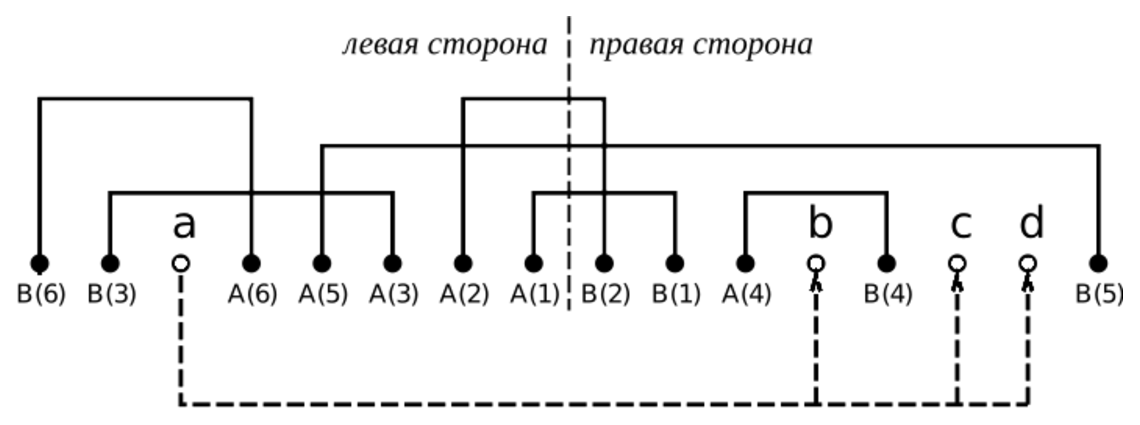
\includegraphics[scale=0.55]{Figs/Probability/labeling-ru}
\end{figure} 

Используя индукцию по $j$, легко доказать, что после того, как выбраны $A(j)$ и $B(j)$, либо одинаковое количество точек было выбрано на каждой из сторон (в случае если $A(j) < B(j)$), либо на левой стороне было выбрано на две точки больше (в случае если $A(j) > B(j)$).

После того, как мы обозначили точки $A(n-2)$ и $B(n-2)$, остаётся четыре необозначенных точки концов интервалов, назовём их $a<b<c< d$.
Мы утверждаем, что из трёх равновероятных способов разбиения этих точек на пары, два приведут к «больш\'{о}му» интервалу, пересекающему все остальные, а один способ --- нет.

В случае если $A(n-2) < B(n-2)$, точки $a$ и $b$ находятся слева, а $c$ и $d$ --- справа;
в противном случае только $a$ находится слева.
В любом случае, все внутренние концы интервалов лежат между точками $a$ и $c$, иначе одна из них была бы выбрана.
Из этого следует, что интервал $[a,c]$ пересекает все остальные, и точно также $[a,d]$.
То есть, если $a$ не в паре с $b$, то у нас большой интервал.

Допустим, напротив, что наши пары именно $[a, b]$ и $[c, d]$.
Ни одна из них не может быть большим интервалом, так как они не пересекаются с друг другом.
Предположим теперь, что существует другой большой интервал, скажем $[e,f]$ с концами $A(j)$ и $B(j)$.

Если точки $a$ и $b$ находятся слева, внутренние концы $A(j)$ лежат между $b$ и $c$, таким образом $[e, f]$ не может пересекать оба интервала $[a, b]$ и $[c, d]$, что противоречит нашему предположению.

В оставшемся случае, так как $[e, f]$ пересекает $[c, d]$, $f$ является внешним концом интервала. 
В этом случае $f=B(j)$, то есть отрезок $[e, f]$ ушёл направо.
Поскольку последняя выбранная пара точек ушла налево, существует $k>j$, для которого $A(k)>B(k)$ и $A(k-1)<B(k-1)$.
В этом случае $A(k)$ лежит слева и значит $A(k) < A(j)$, так как $A(k)$ --- левосторонняя внутренняя точка, выбранная позже.
Тогда $[A(j), B(j)]$ не пересекает $[B(k), A(k)]$; это последнее противоречие доказывает наше утверждение.
\heart

Используя данное рассуждение с чуть большей аккуратностью, можно доказать, что 
для $k < n$ , вероятность того, что в семействе случайных $n$ интервалов найдётся, по меньшей мере, $k$ интервалов, которые пересекают все остальные, равна
\[\frac{2^k}{\binom{2k+1} k}\]
и она не зависит от $n$.
Здесь $\binom n k$ означает \emph{биноминальный коэффициент}, то есть число подмножеств размера $k$ из множества размера $n$, и он равен $n(n-1)(n-2)\cdots(n-k+1) /(k(k-1)(k-2)\cdots1)$.
